\documentclass[tikz,border=2pt]{standalone}
\usepackage{amsmath}
\usetikzlibrary{arrows.meta}
\begin{document}
% Given N(60) = 5, the arrival times are five Unif([0,60]) draws sorted: draws 37.2, 9, 54.6, 24, 16.2
% (upper line, draw order) become A_1..A_5 = 9, 16.2, 24, 37.2, 54.6, where the count N(s) steps up by one.
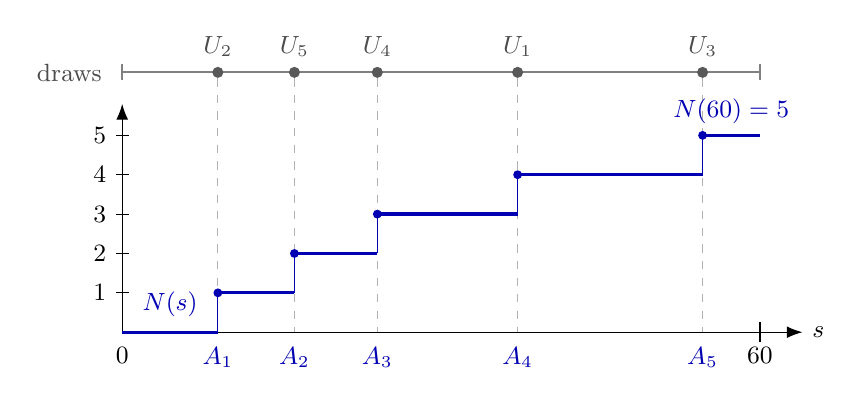
\begin{tikzpicture}[font=\small, >={Latex[length=2mm]}, x=0.135cm, y=0.5cm]
  % upper line: unsorted uniform draws
  \draw[gray, thick] (0,6.6) -- (60,6.6);
  \draw[gray, thick] (0,6.4) -- (0,6.8);
  \draw[gray, thick] (60,6.4) -- (60,6.8);
  \node[gray!60!black, anchor=east] at (-1,6.6) {draws};
  \foreach \u/\i in {37.2/1, 9/2, 54.6/3, 24/4, 16.2/5} {
    \draw[gray!60, dashed] (\u,6.45) -- (\u,0);
    \fill[gray!70!black] (\u,6.6) circle (2pt);
    \node[gray!60!black, anchor=south] at (\u,6.75) {$U_{\i}$};
  }
  % axes
  \draw[->] (0,0) -- (64,0) node[anchor=west] {$s$};
  \draw[->] (0,0) -- (0,5.8);
  \foreach \n in {1,...,5} \draw (0.6,\n) -- (-0.6,\n) node[anchor=east] {$\n$};
  \node[anchor=north] at (0,-0.15) {$0$};
  \node[anchor=north] at (60,-0.15) {$60$};
  \draw (60,0.25) -- (60,-0.25);
  % sorted arrival times
  \foreach \a/\k in {9/1, 16.2/2, 24/3, 37.2/4, 54.6/5} {
    \node[blue!70!black, anchor=north] at (\a,-0.15) {$A_{\k}$};
  }
  % counting process N(s)
  \draw[blue!70!black, very thick] (0,0) -- (9,0);
  \draw[blue!70!black, very thick] (9,1) -- (16.2,1);
  \draw[blue!70!black, very thick] (16.2,2) -- (24,2);
  \draw[blue!70!black, very thick] (24,3) -- (37.2,3);
  \draw[blue!70!black, very thick] (37.2,4) -- (54.6,4);
  \draw[blue!70!black, very thick] (54.6,5) -- (60,5);
  \foreach \a/\n in {9/1, 16.2/2, 24/3, 37.2/4, 54.6/5} {
    \draw[blue!70!black, thin] (\a,\n-1) -- (\a,\n);
    \fill[blue!70!black] (\a,\n) circle (1.6pt);
  }
  \node[blue!70!black, anchor=south west] at (1,0.15) {$N(s)$};
  \node[blue!70!black, anchor=south] at (57.3,5.05) {$N(60)=5$};
\end{tikzpicture}
\end{document}
